\documentclass{ximera}

\newcommand{\RR}{\mathbb R}
\renewcommand{\d}{\,d}
\newcommand{\dd}[2][]{\frac{d #1}{d #2}}
\renewcommand{\l}{\ell}
\newcommand{\ddx}{\frac{d}{dx}}
\newcommand{\dfn}{\textbf}
\newcommand{\eval}[1]{\bigg[ #1 \bigg]}


\outcome{State and use Stokes' theorem.}

\title[Dig-In:]{Stokes' theorem}

\begin{document}
\begin{abstract}
  We introduce Stokes' theorem.
\end{abstract}
\maketitle

Our final fundamental theorem of calculus is Stokes'
theorem. Historically speaking, Stokes' theorem was discovered after
both Green's theorem and the divergence theorem. Its application is
probably the most obscure, with the primary applications being rooted
in electricity-and-magnetism and fluid dynamics.

Nevertheless, once we know Stokes' theorem, we can view it as a direct
generalization of Green's theorem.

\begin{theorem}[Stokes' Theorem]\index{Stokes' Theorem}
  If the components of $\vec{F}:\R^3\to\R^3$ have continuous partial
  derivatives and $\partial R$ is a boundary of a closed surface $R$
  and $\vec{p}(t)$ parameterizes $\partial R$ in a counterclockwise
  direction with the interior on the left, then:
  \[
  \iint_R (\curl \vec{F})\dotp \uvec{n}\d S = \oint_{\partial R}
  \vec{F}\dotp\d\vec{p}
  \]
\end{theorem}

If we compare the conclusion of Stokes' theorem to the conclusion of
Green's theorem, we see that they are quite similar:
  \[
  \underbrace{\iint_R \curl\vec{F}\d A = \oint_{\partial R} \vec{F}\dotp\d\vec{p}}_{\text{Green's Theorem}}\qquad \underbrace{\iint_R (\curl \vec{F})\dotp \uvec{n}\d S = \oint_{\partial R}
  \vec{F}\dotp\d\vec{p}}_{\text{Stokes' Theorem}}
  \]

In essence, Green's theorem is nothing more than Stokes' theorem when
we assume that the surface is restricted to the $(x,y)$-plane. Like
the divergence theorem, one application of Stokes' theorem is to
transform a difficult integral into an easier one.

\begin{example}
  Consider the line integral
  \[
  \oint_C (x-y)\d x +(x-2y+z) \d y + (3x+z) \d z
  \]
  where $C$ is parameterized by $\vec{p}(t) =
  \vector{\cos(t),\sin(t),3}$, $0\le t<2\pi$. Compute this integral
  using Stokes' theorem.
  \begin{explanation}
    Let $R$ be the surface bounded by $C$, so in this case $C =
    \partial R$. Moreover, set
    \[
    \vec{F}(x,y,z) = \vector{x-y,x-2y+z,3x+z}.
    \]
    Now we may write:
    \[
    \oint_C (x-y)\d x +(x-2y+z) \d y + (3x+z) \d z = \oint_{\partial R} \vec{F}\dotp\d\vec{p} 
    \]
    and Stokes' theorem says:
    \[
    \oint_{\partial R} \vec{F}\dotp\d\vec{p}  = \iint_R (\curl \vec{F})\dotp \uvec{n}\d S
    \]
    Write with me,
    \begin{align*}
      \curl F(x,y,z) = \vector{\answer[given]{-1},\answer[given]{-3},\answer[given]{2}}\\
      \uvec{n} = \vector{\answer[given]{0},\answer[given]{0},\answer[given]{1}}.
    \end{align*}
    Hence
    \[
    \iint_R \vector{-1,-3,2}\dotp \vector{0,0,1}\d S = \answer[given]{2}\iint_R \d S
    \]
    but
    \[
    \iint_R \d S = \answer[given]{\pi}
    \]
    Hence
    \[
    \oint_C (x-y)\d x +(x-2y+z) \d y + (3x+z) \d z =\answer[given]{2\pi}.
    \]
  \end{explanation}
\end{example}


%% \section{Observations from Stokes' theorem}
%% Explain how to change the surface
%% fact that circulation on any closed surface is zero.
%% In particular, if the boundry is contained to a plane, the avg value of the surface normals is exactly the normal vector to the plane



\begin{example}
  Consider the surface integral
  \[
  \iint_R (\curl \vec{F})\dotp \uvec{n}\d S
  \]
  where
  \[
  \vec{F}(x,y,z) = \vector{-y,0,z^2}
  \]
  and $R$ is the upper hemisphere of the sphere:
  \[
  x^2 + y^2 + z^2 = 9
  \]
  Compute this integral using Stokes' theorem.
  \begin{explanation}
    Note that the boundary of the sphere is \textbf{identical} to the boundary of the disk
    \[
    \vec{p}(t) = \vector{3\cos(t),3\sin(t),0}
    \]
    where $0\le t<2\pi$. Hence we may dispense with our ``upper
    hemisphere'' and simply work with the disk of radius $3$.
    Write with me,
    \[
    \curl F(x,y,z) = \vector{\answer[given]{0},\answer[given]{0},\answer[given]{1}}
    \]
    Hence
    \begin{align*}
      \iint_R \vector{0,0,1}\dotp \vector{0,0,1}\d S &= \iint_R \d S\\
      \answer[given]{9\pi}.
    \end{align*}
    By Stokes' theorem this is equal to the integral we desire.
  \end{explanation}
\end{example}




\section{Our final fundamental theorem of calculus}

How is Stokes' Theorem a fundamental theorem of calculus? Well
consider this:
\begin{image}
  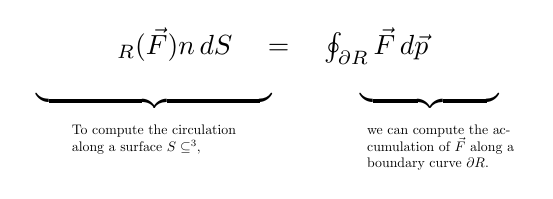
\begin{tikzpicture}
    \node[inner sep=0pt] at (0,0) {$\iint_R (\curl\vec{F})\dotp \uvec{n}\d S\quad =\quad \oint_{\partial R} \vec{F}\dotp\d\vec{p}$};

    \node at (-1.5,-.7) {$\underbrace{\hspace{8.5em}}$};

    \node at (2,-.7) {$\underbrace{\hspace{5em}}$};

    \node[below,inner sep=0pt,text width=5cm,scale=.5] at (-1.3,-1)
         {To compute the circulation along a surface $S\subseteq\R^3$, };

    \node[below,inner sep=0pt,text width=4cm,scale=.5] at (2.2,-1) {we can compute the accumulation of $\vec{F}$ along a boundary curve $\partial R$.};
  \end{tikzpicture}
\end{image}


Are there no more fundamental theorems of calculus? Well, there are,
but as you will see if you continue your study of mathematics, they
are all generalizations of the theorems we already know.


For some interesting extra reading check out:
\begin{itemize}
\item \link[\textit{The History of Stokes' Theorem}, V.J.\ Katz,
  Mathematics Magazine, May
  1979.]{http://www.jstor.org/stable/2690275}
\end{itemize}


\end{document}
